\documentclass[11pt]{beamer}
\usetheme{Warsaw}
\usepackage[frenchb]{babel}
\usepackage[T1]{fontenc}
\usepackage[utf8]{inputenc}
\usepackage{listings}
\usepackage{amsmath}
\usepackage{amsfonts}
\usepackage{amssymb}
\usepackage{forest}
\usepackage{xcolor}

\definecolor{folderbg}{RGB}{124,166,198}
\definecolor{folderborder}{RGB}{110,144,169}

\def\Size{4pt}
\tikzset{
  folder/.pic={
    \filldraw[draw=folderborder,top color=folderbg!50,bottom color=folderbg]
      (-1.05*\Size,0.2\Size+5pt) rectangle ++(.75*\Size,-0.2\Size-5pt);  
    \filldraw[draw=folderborder,top color=folderbg!50,bottom color=folderbg]
      (-1.15*\Size,-\Size) rectangle (1.15*\Size,\Size);
  }
}

\lstset{language=C++,
	basicstyle=\tiny\ttfamily,
	keywordstyle=\color{blue}\ttfamily,
	stringstyle=\color{red}\ttfamily,
	commentstyle=\color{green}\ttfamily,
	morecomment=[l][\color{magenta}]{\#},
	breaklines=true,
	breakatwhitespace=true
}

\author{Lazare Lucas - Pinard Maxime}
\title{Présentation TZ20}
%\setbeamercovered{transparent} 
%\setbeamertemplate{navigation symbols}{} 
%\logo{} 
\institute{UTBM} 
\date{\today} 
\subject{TZ20} 
\begin{document}

\begin{frame}
	\titlepage{}
\end{frame}

\begin{frame}
	\tableofcontents{}
\end{frame}

\section{Objectifs}

	\begin{frame}
		\frametitle{Objectifs}
		\begin{itemize}
			\item{} Restriction d'accès
			\item{} Dossier privé et publique
			\item{} Affichage fonction \textit{ls}
			\item{} Suppression des fichier (24h)
			\item{} Logs de connexion
			\item{} Changement de mot de passe
			\item{} Descriptions de fichiers
			\item{} Création de nouveaux comptes
			\item{} Configuration du serveur
		\end{itemize}
	\end{frame}

\section{Problèmes}

	\begin{frame}
		\frametitle{Problèmes}
		\begin{itemize}
			\item{} Communication client - serveur
			\item{} Interprétation des commandes
			\item{} Gerer les restrictions d'accès
			\item{} Récupérer la liste des dossiers et fichiers présents dans un dossier
			\item{} Stocker des informations à propos des dossiers et fichiers uploadés
			\item{} Afficher des informations de façon ergonomique/lisible
			\item{} Envoyer des mails via un programme
			\item{} Créer, gérer et utiliser la configuration du serveur
			\item{} Permettre au client de télécharger / uploader un dossier complet
		\end{itemize}
	\end{frame}

\section{Solutions}
	\subsection{Architecture}

		\begin{frame}
			\frametitle{Architecture}
			%\framesubtitle{avec un exemple de sous-titre}
			\begin{forest}
			  for tree={
			    font=\ttfamily,
			    grow'=0,
			    child anchor=west,
			    parent anchor=south,
			    anchor=west,
			    calign=first,
			    inner xsep=7pt,
			    edge path={
			      \noexpand\path [draw, \forestoption{edge}]
			      (!u.south west) +(7.5pt,0) |- (.child anchor) pic {folder} \forestoption{edge label};
			    },
			    before typesetting nodes={
			      if n=1
			        {insert before={[,phantom]}}
			        {}
			    },
			    fit=band,
			    before computing xy={l=15pt},
			  }  
			[server execution folder
			  [Downloading\_Threads
			  ]
			  [FilesData
			  ]
			  [IPList
			  ]
			  [Public
			  ]
			  [Private
			  ]
			  [ToConf
			  ]
			  [UsersData
			  ]
			]
			\end{forest}
		\end{frame}

	\subsection{Interface}

		\begin{frame}
			\frametitle{Interface}
			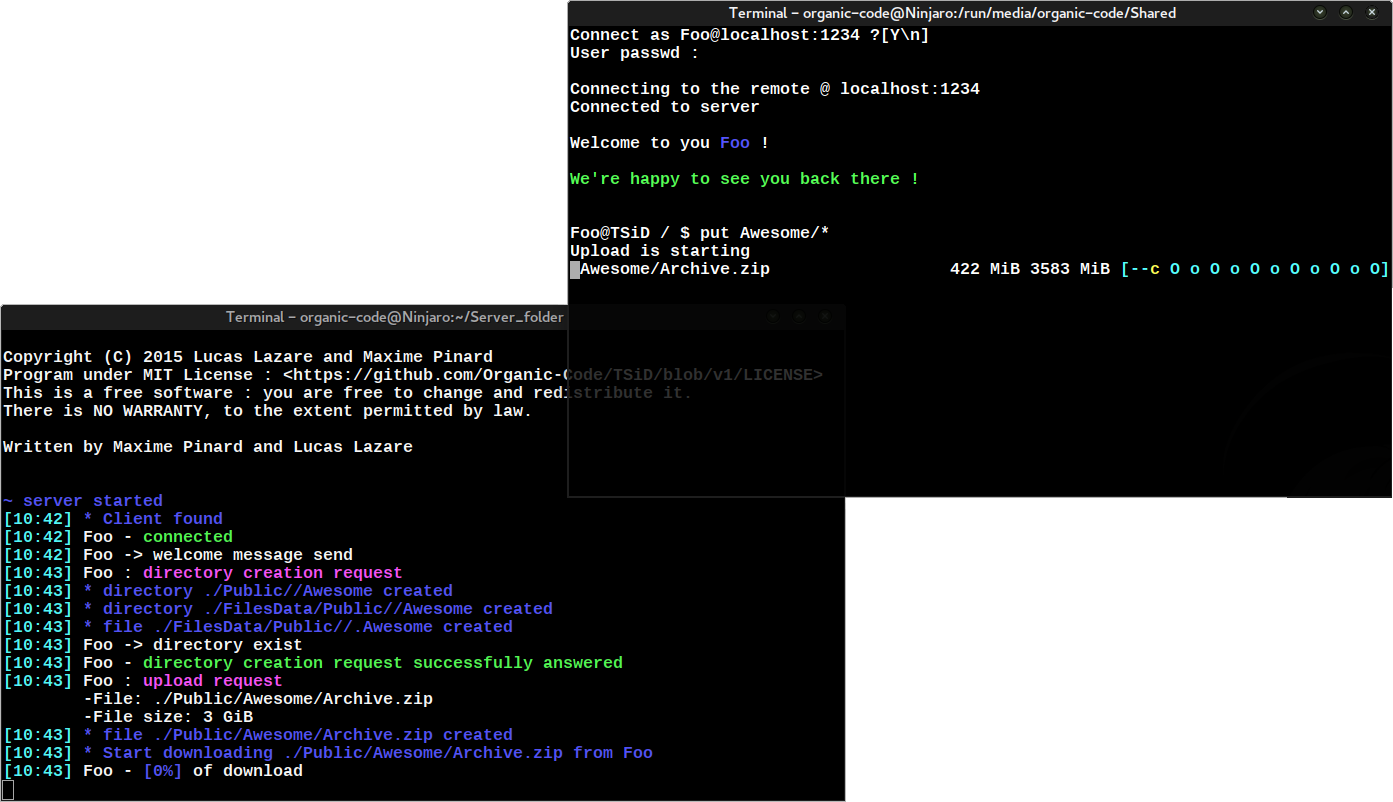
\includegraphics[width=\linewidth]{interface}
		\end{frame}

\section{Exemple}
	\subsection{Serveur: a\_retrieveData}

		\begin{frame}
			\frametitle{Serveur: a\_retrieveData}
			\begin{lstlisting}
//error
client.packet.clear();
client.packet << UnknownIssue;
client.socket.send(client.packet);
tprint();
std::cout << client.name() << " -> There was an error [...]" << std::endl;

bool a_retrieveData(Client& client){

    unsigned int file_size;
    unsigned int bytes_per_packet;

    if( !(client.packet >> file_size >> bytes_per_packet) ){
        //error
        return false;
    }
    std::cout << "\t-File: " << client.path << std::endl;

    if( file_size == 0 ){
        //error
        return false;
    }
\end{lstlisting}
		\end{frame}

		\begin{frame}
			\frametitle{Serveur: a\_retrieveData}
			\begin{lstlisting}
    if(file_size < 1024 ){
        std::cout << "\t-File size: " << file_size << " B" << std::endl;
    }
    
    else if(file_size < 1024 * 1024 ){
        std::cout << "\t-File size: " << file_size/1024 << " KiB" << std::endl;
    }
    
    else if(file_size < 1024 * 1024 * 1024 ){
        std::cout << "\t-File size: " << file_size/(1024 * 1024)<< " MiB" << std::endl;
    }
    
    else{
        std::cout << "\t-File size: " << file_size/(1024 * 1024 * 1024)<< " GiB" << std::endl;
    }
\end{lstlisting}
		\end{frame}

		\begin{frame}
			\frametitle{Serveur: a\_retrieveData}
			\begin{lstlisting}
    client.packet.clear();

    switch(createFile(client.path)){
        
        case AlreadyExist:
            client.packet << AlreadyExist;
            client.socket.send(client.packet);
            tprint();
            std::cout << client.name() << " -> File already exists" << std::endl;
            return false;
            break;

        case UnknownIssue:
            //error
            return false;
            break;

        default:
            break;
    }
\end{lstlisting}
		\end{frame}

		\begin{frame}
			\frametitle{Serveur: a\_retrieveData}
			\begin{lstlisting}
    std::ofstream output_file ( client.path.c_str(), std::ios::binary | std::ios::out );

    unsigned int loop_number(file_size/bytes_per_packet);
    char* input_data_array = new char[bytes_per_packet];
    sf::Int8 input_data;
    unsigned char percentage_count(0);

    client.packet.clear();
    client.packet << ServerReady;
    client.socket.send(client.packet);

    tprint();
    setColors("light blue");
    std::cout << "* Start downloading " << client.path << " from " << client.name() << std::endl;
    setColors("reset");
\end{lstlisting}
		\end{frame}

		\begin{frame}
			\frametitle{Serveur: a\_retrieveData}
			\begin{lstlisting}
    for( unsigned int i(0) ; i<loop_number ; ++i){
        
        client.packet.clear();

        if(client.socket.receive( client.packet ) == sf::Socket::Disconnected){
            //error
            output_file.close();
            removeFile(client.path);
            return false;
        }

        for( unsigned int j(0) ; j<bytes_per_packet ; ++j ){
            client.packet >> input_data;
            input_data_array[j]=static_cast<char>(input_data);
        }

        output_file.write( input_data_array, bytes_per_packet );

        if( static_cast<unsigned char>(100*i/loop_number) > percentage_count ){
            tprint();
            std::cout << client.name() << " - ";
            setColors("light blue");
            std::cout << "[" << static_cast<short>(percentage_count) << "%]";
            setColors("reset");
            std::cout << " of download" << std::endl;
            percentage_count = static_cast<unsigned char>(percentage_count + 25);
        }
    }
\end{lstlisting}
		\end{frame}

		\begin{frame}
			\frametitle{Serveur: a\_retrieveData}
			\begin{lstlisting}
    file_size -= loop_number * bytes_per_packet;
    if( file_size > 0 ){
        
        client.packet.clear();
        if(client.socket.receive( client.packet ) == sf::Socket::Disconnected){
            //error
            output_file.close();
            removeFile(client.path);
            return false;
        }

        for( unsigned int j(0) ; j < client.packet.getDataSize() ; ++j){
            client.packet >> input_data;
            output_file << static_cast<char>(input_data);
        }
    }
\end{lstlisting}
		\end{frame}

		\begin{frame}
			\frametitle{Serveur: a\_retrieveData}
			\begin{lstlisting}
    output_file.close();

    tprint();
    std::cout << client.name() << " - ";
    setColors("light blue");
    std::cout << "[100%]";
    setColors("reset");
    std::cout << " Transfer terminated successfully" << std::endl;
    createInformationFile(client.path, client.name());
    delete[] input_data_array;
    return true;
}
\end{lstlisting}
		\end{frame}

	\subsection{Serveur: createInformationFile}

		\begin{frame}
			\frametitle{Serveur: createInformationFile}
			\begin{lstlisting}
char createInformationFile(std::string path, std::string user_name){

    std::string info_path = "./FilesData" + path.substr(1, std::string::npos); //add "./FilesData" at the begening

    if( fileExist(info_path) ){
        setColors("light red");
        std::cout << "\t-The informations file already exist" << std::endl;
        setColors("reset");
        return AlreadyExist;
    }

    if(isFolder(path)){
        createDirectory(info_path);
    }
\end{lstlisting}
		\end{frame}

		\begin{frame}
			\frametitle{Serveur: createInformationFile}
			\begin{lstlisting}
    info_path = info_path.insert(info_path.find_last_of("/") + 1,"."); //insert '.' before the filename
    createFile(info_path);
    std::ofstream file ( info_path.c_str(), std::ios::binary | std::ios::out );

    if( file.fail() ){
        file.close();
        std::cout << "\t-";
        setColors("light red");
        std::cout << "Error writting in the informations file" << std::endl;
        setColors("reset");
        return UnknownIssue;
    }

    file << formatedTime() << std::endl;
    file << user_name << std::endl;
    file.close();
    return Created;
}
\end{lstlisting}
		\end{frame}

	\subsection{Client: sendData}
	
		\begin{frame}
			\frametitle{Client: sendData}
			\begin{lstlisting}
bool sendData(sf::TcpSocket& server, std::string const& current_directory) {

	std::ifstream input_file;
	unsigned int file_size;

	std::cin.ignore();
	std::string filename;
	std::getline(std::cin, filename);

	if (filename.back() == '*') {
		filename.pop_back();
		filename.pop_back();
		return recursiveUpload( server, current_directory, ".", filename );
	}

	if (!startUpload(input_file, file_size, server, current_directory, filename)) {

		std::cout << "Could not send the file" << std::endl;
		return false;
	}
	return uploadFile( server, input_file, file_size, filename );
}
\end{lstlisting}

		\end{frame}

	\subsection{Client: startUpload}
	
		\begin{frame}
			\frametitle{Client: startUpload}
			\begin{lstlisting}
bool startUpload(std::ifstream& infile, unsigned int& file_size, sf::TcpSocket& server, std::string const& dir, std::string filename)

	std::string directory(dir);
	formatDir(directory);
	if (isFolder(filename)) {
		std::cout << "You are trying to upload a folder... (maybe you forgot to add * ?)"
			<< std::endl;
		return false;
	}
	file_size = getFileLength( filename );
	infile.open( filename.c_str(), std::ios::binary | std::ios::in);
	if( file_size == 0 || infile.fail() ) {
		std::cout << "There was a problem reading the file : " << filename << " (maybe that this file is empty ?)" << std::endl;
		return false;
	}
	
	sf::Packet packet;
	packet << (directory+'/'+formatPath(filename)) << Upload << file_size << NB_BYTE_PER_PACKET;
	server.send(packet);
	packet.clear();

	int server_state;
	server.receive(packet);
	if( packet.getDataSize() > sizeof( int ) || !(packet >> server_state) ){

		std::cout << "There was an error retrieving server state" << std::endl;
		return false;
	}
	return interpretServerAns(static_cast<char>(server_state));
\end{lstlisting}

		\end{frame}
\end{document}
